\documentclass[12pt,a4paper]{article}

\usepackage[a4paper,text={16.5cm,25.2cm},centering, margin=1in]{geometry}

\usepackage[scale=0.95]{FiraMono}
\usepackage[utf8]{inputenc}
\usepackage[T1]{fontenc}
\usepackage{mathpazo}

\usepackage{amssymb,amsmath}
\usepackage{bm}
\usepackage{graphicx}
\usepackage{microtype}
\usepackage{hyperref}
\setlength{\parindent}{0pt}
\setlength{\parskip}{1.2ex}

\usepackage{fvextra}
\DefineVerbatimEnvironment{Highlighting}{Verbatim}{breaklines,commandchars=\\\{\}}

\setcounter{secnumdepth}{0}

\hypersetup
       {   pdfauthor = { Andrew Scacchi (ads339) },
           pdftitle={ BEE 4750/5750 Homework 3 },
           colorlinks=TRUE,
           linkcolor=black,
           citecolor=blue,
           urlcolor=blue
       }

\title{ BEE 4750/5750 Homework 3 }

\author{ Andrew Scacchi (ads339) }

\date{ 2022-10-22 }

\usepackage{upquote}
\usepackage{listings}
\usepackage{xcolor}
\lstset{
    basicstyle=\ttfamily\footnotesize,
    upquote=true,
    breaklines=true,
    breakindent=0pt,
    keepspaces=true,
    showspaces=false,
    columns=fullflexible,
    showtabs=false,
    showstringspaces=false,
    escapeinside={(*@}{@*)},
    extendedchars=true,
}
\newcommand{\HLJLt}[1]{#1}
\newcommand{\HLJLw}[1]{#1}
\newcommand{\HLJLe}[1]{#1}
\newcommand{\HLJLeB}[1]{#1}
\newcommand{\HLJLo}[1]{#1}
\newcommand{\HLJLk}[1]{\textcolor[RGB]{148,91,176}{\textbf{#1}}}
\newcommand{\HLJLkc}[1]{\textcolor[RGB]{59,151,46}{\textit{#1}}}
\newcommand{\HLJLkd}[1]{\textcolor[RGB]{214,102,97}{\textit{#1}}}
\newcommand{\HLJLkn}[1]{\textcolor[RGB]{148,91,176}{\textbf{#1}}}
\newcommand{\HLJLkp}[1]{\textcolor[RGB]{148,91,176}{\textbf{#1}}}
\newcommand{\HLJLkr}[1]{\textcolor[RGB]{148,91,176}{\textbf{#1}}}
\newcommand{\HLJLkt}[1]{\textcolor[RGB]{148,91,176}{\textbf{#1}}}
\newcommand{\HLJLn}[1]{#1}
\newcommand{\HLJLna}[1]{#1}
\newcommand{\HLJLnb}[1]{#1}
\newcommand{\HLJLnbp}[1]{#1}
\newcommand{\HLJLnc}[1]{#1}
\newcommand{\HLJLncB}[1]{#1}
\newcommand{\HLJLnd}[1]{\textcolor[RGB]{214,102,97}{#1}}
\newcommand{\HLJLne}[1]{#1}
\newcommand{\HLJLneB}[1]{#1}
\newcommand{\HLJLnf}[1]{\textcolor[RGB]{66,102,213}{#1}}
\newcommand{\HLJLnfm}[1]{\textcolor[RGB]{66,102,213}{#1}}
\newcommand{\HLJLnp}[1]{#1}
\newcommand{\HLJLnl}[1]{#1}
\newcommand{\HLJLnn}[1]{#1}
\newcommand{\HLJLno}[1]{#1}
\newcommand{\HLJLnt}[1]{#1}
\newcommand{\HLJLnv}[1]{#1}
\newcommand{\HLJLnvc}[1]{#1}
\newcommand{\HLJLnvg}[1]{#1}
\newcommand{\HLJLnvi}[1]{#1}
\newcommand{\HLJLnvm}[1]{#1}
\newcommand{\HLJLl}[1]{#1}
\newcommand{\HLJLld}[1]{\textcolor[RGB]{148,91,176}{\textit{#1}}}
\newcommand{\HLJLs}[1]{\textcolor[RGB]{201,61,57}{#1}}
\newcommand{\HLJLsa}[1]{\textcolor[RGB]{201,61,57}{#1}}
\newcommand{\HLJLsb}[1]{\textcolor[RGB]{201,61,57}{#1}}
\newcommand{\HLJLsc}[1]{\textcolor[RGB]{201,61,57}{#1}}
\newcommand{\HLJLsd}[1]{\textcolor[RGB]{201,61,57}{#1}}
\newcommand{\HLJLsdB}[1]{\textcolor[RGB]{201,61,57}{#1}}
\newcommand{\HLJLsdC}[1]{\textcolor[RGB]{201,61,57}{#1}}
\newcommand{\HLJLse}[1]{\textcolor[RGB]{59,151,46}{#1}}
\newcommand{\HLJLsh}[1]{\textcolor[RGB]{201,61,57}{#1}}
\newcommand{\HLJLsi}[1]{#1}
\newcommand{\HLJLso}[1]{\textcolor[RGB]{201,61,57}{#1}}
\newcommand{\HLJLsr}[1]{\textcolor[RGB]{201,61,57}{#1}}
\newcommand{\HLJLss}[1]{\textcolor[RGB]{201,61,57}{#1}}
\newcommand{\HLJLssB}[1]{\textcolor[RGB]{201,61,57}{#1}}
\newcommand{\HLJLnB}[1]{\textcolor[RGB]{59,151,46}{#1}}
\newcommand{\HLJLnbB}[1]{\textcolor[RGB]{59,151,46}{#1}}
\newcommand{\HLJLnfB}[1]{\textcolor[RGB]{59,151,46}{#1}}
\newcommand{\HLJLnh}[1]{\textcolor[RGB]{59,151,46}{#1}}
\newcommand{\HLJLni}[1]{\textcolor[RGB]{59,151,46}{#1}}
\newcommand{\HLJLnil}[1]{\textcolor[RGB]{59,151,46}{#1}}
\newcommand{\HLJLnoB}[1]{\textcolor[RGB]{59,151,46}{#1}}
\newcommand{\HLJLoB}[1]{\textcolor[RGB]{102,102,102}{\textbf{#1}}}
\newcommand{\HLJLow}[1]{\textcolor[RGB]{102,102,102}{\textbf{#1}}}
\newcommand{\HLJLp}[1]{#1}
\newcommand{\HLJLc}[1]{\textcolor[RGB]{153,153,119}{\textit{#1}}}
\newcommand{\HLJLch}[1]{\textcolor[RGB]{153,153,119}{\textit{#1}}}
\newcommand{\HLJLcm}[1]{\textcolor[RGB]{153,153,119}{\textit{#1}}}
\newcommand{\HLJLcp}[1]{\textcolor[RGB]{153,153,119}{\textit{#1}}}
\newcommand{\HLJLcpB}[1]{\textcolor[RGB]{153,153,119}{\textit{#1}}}
\newcommand{\HLJLcs}[1]{\textcolor[RGB]{153,153,119}{\textit{#1}}}
\newcommand{\HLJLcsB}[1]{\textcolor[RGB]{153,153,119}{\textit{#1}}}
\newcommand{\HLJLg}[1]{#1}
\newcommand{\HLJLgd}[1]{#1}
\newcommand{\HLJLge}[1]{#1}
\newcommand{\HLJLgeB}[1]{#1}
\newcommand{\HLJLgh}[1]{#1}
\newcommand{\HLJLgi}[1]{#1}
\newcommand{\HLJLgo}[1]{#1}
\newcommand{\HLJLgp}[1]{#1}
\newcommand{\HLJLgs}[1]{#1}
\newcommand{\HLJLgsB}[1]{#1}
\newcommand{\HLJLgt}[1]{#1}


\begin{document}

\maketitle

%  This setups the environment and installs packages, but doesn't appear in the generated document 
%  You shouldn't need to modify this 


% - this block is hidden, but stores the generator and demand data; you can use a dataframe to combine these or refactor as you'd like 


\section{Problem 1}

\begin{lstlisting}
(*@\HLJLnB{julia>}@*) (*@\HLJLk{using}@*) (*@\HLJLn{JuMP}@*)

(*@\HLJLnB{julia>}@*) (*@\HLJLk{using}@*) (*@\HLJLn{Plots}@*)

(*@\HLJLnB{julia>}@*) (*@\HLJLk{using}@*) (*@\HLJLn{HiGHS}@*)S
\end{lstlisting}

\subsection{Problem 1.1}
The decision variables for this model include the ultimate production capacity for each energy generation type, and the actual energy output at a given time for each generator constructed.

Theoretical Production Capacity (MW) = $x_G$ with G representing the type of energy generated. G = \{Geothermal, Coal, CCGT, CT, Wind, Solar\}

Energy Output at time t (MW) = $y_{G,t}$

Nonserved energy values (MW) at a particular time t = $n_t$

\subsection{Problem 1.2}
The objective function  to minimize total costs of building and operating the expansion plan is to minimize the annual capital investment cost, O\&M costs, and the unserved energy cost,  which all aggregate to Total Cost $Z$. This can be expressed mathematically as:

Initial investment cost for plant $G$ (per MW-year) = $C_G^{INV}$

O\&M Costs (per MWh) for plant $G$ = $C_G^{OP}$

Unserved Energy costs  = $C_t^{NSE}$ 

Time passed (for now is equal to a year but so that no hardcoding) = $L_t$

Overall evaluate out to:

\[
min Z = \sum_G C_G^{INV} x_G + 365 \sum_G \sum_t L_t C_G^{OP} y_{G,t} + 365 \sum_t L_t C_t^{NSE} n_t
\]
\subsection{Problem 1.3}
There exist several physical constraints on this system. The first one is that no generator can produce more energy than it is physically capable of:

\[
y_{G,t}\ensuremath{\leq} x_G CF_G
\]
Additionally, demand at time t $D_t$ has to equal total energy production at t + unserved demand at t:

\[
\sum_G y_{G,t} + n_t = D_t
\]
Lastly, production outputs cannot be negative:

\[
x_G \ensuremath{\geq} 0 \\
y_{G,t} \ensuremath{\geq} 0 \\
n_t \ensuremath{\geq} 0 \\
\]
My set of constraints is complete as all physical limitations (need to produce between 0 and x\_G at time t) are accounted for. Additionally, unmet demand has to be positive, and the sum of met and unmet demand sums to the total demand from clients. If unmet demand is 0 or more, then  it is impossible to produce moreelectriity than is required, making a 4th constraint obsolete.

\subsection{Problem 1.4}

\begin{lstlisting}
(*@\HLJLnB{julia>}@*) (*@\HLJLn{Generators}@*) (*@\HLJLoB{=}@*) (*@\HLJLp{[}@*)(*@\HLJLs{"{}Geothermal"{}}@*)(*@\HLJLp{,}@*) (*@\HLJLs{"{}Coal"{}}@*)(*@\HLJLp{,}@*) (*@\HLJLs{"{}CCGT"{}}@*)(*@\HLJLp{,}@*) (*@\HLJLs{"{}CT"{}}@*)(*@\HLJLp{,}@*) (*@\HLJLs{"{}Wind"{}}@*)(*@\HLJLp{,}@*) (*@\HLJLs{"{}Solar"{}}@*)(*@\HLJLp{];}@*)

(*@\HLJLnB{julia>}@*) (*@\HLJLn{G}@*) (*@\HLJLoB{=}@*) (*@\HLJLni{1}@*)(*@\HLJLoB{:}@*)(*@\HLJLnf{length}@*)(*@\HLJLp{(}@*)(*@\HLJLn{Generators}@*)(*@\HLJLp{);}@*)

(*@\HLJLnB{julia>}@*) (*@\HLJLn{T}@*)(*@\HLJLoB{=}@*) (*@\HLJLn{hours}@*)(*@\HLJLp{;}@*)

(*@\HLJLnB{julia>}@*) (*@\HLJLn{Q}@*) (*@\HLJLoB{=}@*) (*@\HLJLnf{Model}@*)(*@\HLJLp{(}@*)(*@\HLJLn{HiGHS}@*)(*@\HLJLoB{.}@*)(*@\HLJLn{Optimizer}@*)(*@\HLJLp{);}@*)

(*@\HLJLnB{julia>}@*) (*@\HLJLn{nseCost}@*) (*@\HLJLoB{=}@*) (*@\HLJLni{1000}@*)(*@\HLJLp{;}@*)

(*@\HLJLnB{julia>}@*) (*@\HLJLnd{@variable}@*)(*@\HLJLp{(}@*)(*@\HLJLn{Q}@*)(*@\HLJLp{,}@*) (*@\HLJLn{x}@*)(*@\HLJLp{[}@*)(*@\HLJLn{G}@*)(*@\HLJLp{]}@*)(*@\HLJLoB{>=}@*)(*@\HLJLni{0}@*)(*@\HLJLp{);}@*)

(*@\HLJLnB{julia>}@*) (*@\HLJLnd{@variable}@*)(*@\HLJLp{(}@*)(*@\HLJLn{Q}@*)(*@\HLJLp{,}@*) (*@\HLJLn{y}@*)(*@\HLJLp{[}@*)(*@\HLJLn{G}@*)(*@\HLJLp{,}@*)(*@\HLJLn{T}@*)(*@\HLJLp{]}@*) (*@\HLJLoB{>=}@*) (*@\HLJLni{0}@*)(*@\HLJLp{);}@*)

(*@\HLJLnB{julia>}@*) (*@\HLJLnd{@variable}@*)(*@\HLJLp{(}@*)(*@\HLJLn{Q}@*)(*@\HLJLp{,}@*) (*@\HLJLn{n}@*)(*@\HLJLp{[}@*)(*@\HLJLn{T}@*)(*@\HLJLp{]}@*) (*@\HLJLoB{>=}@*)(*@\HLJLni{0}@*)(*@\HLJLp{);}@*)

(*@\HLJLnB{julia>}@*) (*@\HLJLnd{@objective}@*)(*@\HLJLp{(}@*)(*@\HLJLn{Q}@*)(*@\HLJLp{,}@*) (*@\HLJLn{Min}@*)(*@\HLJLp{,}@*) (*@\HLJLn{investment{\_}cost}@*)(*@\HLJLoB{{\textquotesingle}*}@*) (*@\HLJLn{x}@*) (*@\HLJLoB{+}@*) (*@\HLJLni{365}@*)(*@\HLJLoB{*}@*)(*@\HLJLp{(}@*)(*@\HLJLnf{sum}@*)(*@\HLJLp{(}@*)(*@\HLJLn{op{\_}cost}@*)(*@\HLJLoB{{\textquotesingle}*}@*)(*@\HLJLn{y}@*)(*@\HLJLp{)}@*) (*@\HLJLoB{+}@*) (*@\HLJLnf{sum}@*)(*@\HLJLp{(}@*)(*@\HLJLn{n}@*)(*@\HLJLp{)}@*)(*@\HLJLoB{*}@*)(*@\HLJLn{nseCost}@*)(*@\HLJLp{))}@*)
457000 x[1] + 268000 x[2] + 85000 x[3] + 62580 x[4] + 92000 x[5] + 92000 x[6] + 8030 y[2,1] + 12775 y[3,1] + 16425 y[4,1] + 8030 y[2,2] + 12775 y[3,2] + 16425 y[4,2] + 8030 y[2,3] + 12775 y[3,3] + 16425 y[4,3] + 8030 y[2,4] + 12775 y[3,4] + 16425 y[4,4] + 8030 y[2,5] + 12775 y[3,5] + 16425 y[4,5] + 8030 y[2,6] + 12775 y[3,6] + 16425 y[4,6] + 8030 y[2,7] + 12775 y[3,7] + 16425 y[4,7] + 8030 y[2,8] + 12775 y[3,8] + 16425 y[4,8] + 8030 y[2,9] + 12775 y[3,9] + 16425 y[4,9] + 8030 y[2,10] + 12775 y[3,10] + 16425 y[4,10] + 8030 y[2,11] + 12775 y[3,11] + 16425 y[4,11] + 8030 y[2,12] + 12775 y[3,12] + 16425 y[4,12] + 8030 y[2,13] + 12775 y[3,13] + 16425 y[4,13] + 8030 y[2,14] + 12775 y[3,14] + 16425 y[4,14] + 8030 y[2,15] + 12775 y[3,15] + 16425 y[4,15] + 8030 y[2,16] + 12775 y[3,16] + 16425 y[4,16] + 8030 y[2,17] + 12775 y[3,17] + 16425 y[4,17] + 8030 y[2,18] + 12775 y[3,18] + 16425 y[4,18] + 8030 y[2,19] + 12775 y[3,19] + 16425 y[4,19] + 8030 y[2,20] + 12775 y[3,20] + 16425 y[4,20] + 8030 y[2,21] + 12775 y[3,21] + 16425 y[4,21] + 8030 y[2,22] + 12775 y[3,22] + 16425 y[4,22] + 8030 y[2,23] + 12775 y[3,23] + 16425 y[4,23] + 8030 y[2,24] + 12775 y[3,24] + 16425 y[4,24] + 365000 n[1] + 365000 n[2] + 365000 n[3] + 365000 n[4] + 365000 n[5] + 365000 n[6] + 365000 n[7] + 365000 n[8] + 365000 n[9] + 365000 n[10] + 365000 n[11] + 365000 n[12] + 365000 n[13] + 365000 n[14] + 365000 n[15] + 365000 n[16] + 365000 n[17] + 365000 n[18] + 365000 n[19] + 365000 n[20] + 365000 n[21] + 365000 n[22] + 365000 n[23] + 365000 n[24]

(*@\HLJLnB{julia>}@*) (*@\HLJLn{available}@*) (*@\HLJLoB{=}@*) (*@\HLJLnf{zeros}@*)(*@\HLJLp{(}@*)(*@\HLJLnf{length}@*)(*@\HLJLp{(}@*)(*@\HLJLn{G}@*)(*@\HLJLp{),}@*) (*@\HLJLnf{length}@*)(*@\HLJLp{(}@*)(*@\HLJLn{T}@*)(*@\HLJLp{));}@*)

(*@\HLJLnB{julia>}@*) (*@\HLJLn{available}@*)(*@\HLJLp{[}@*)(*@\HLJLni{1}@*)(*@\HLJLp{,}@*)(*@\HLJLoB{:}@*)(*@\HLJLp{]}@*) (*@\HLJLoB{.=}@*)(*@\HLJLn{thermal{\_}cf}@*)(*@\HLJLp{[}@*)(*@\HLJLni{1}@*)(*@\HLJLp{];}@*)

(*@\HLJLnB{julia>}@*) (*@\HLJLn{available}@*)(*@\HLJLp{[}@*)(*@\HLJLni{2}@*)(*@\HLJLp{,}@*)(*@\HLJLoB{:}@*)(*@\HLJLp{]}@*) (*@\HLJLoB{.=}@*)(*@\HLJLn{thermal{\_}cf}@*)(*@\HLJLp{[}@*)(*@\HLJLni{2}@*)(*@\HLJLp{];}@*)

(*@\HLJLnB{julia>}@*) (*@\HLJLn{available}@*)(*@\HLJLp{[}@*)(*@\HLJLni{3}@*)(*@\HLJLp{,}@*)(*@\HLJLoB{:}@*)(*@\HLJLp{]}@*) (*@\HLJLoB{.=}@*)(*@\HLJLn{thermal{\_}cf}@*)(*@\HLJLp{[}@*)(*@\HLJLni{3}@*)(*@\HLJLp{];}@*)

(*@\HLJLnB{julia>}@*) (*@\HLJLn{available}@*)(*@\HLJLp{[}@*)(*@\HLJLni{4}@*)(*@\HLJLp{,}@*)(*@\HLJLoB{:}@*)(*@\HLJLp{]}@*) (*@\HLJLoB{.=}@*)(*@\HLJLn{thermal{\_}cf}@*)(*@\HLJLp{[}@*)(*@\HLJLni{4}@*)(*@\HLJLp{];}@*)

(*@\HLJLnB{julia>}@*) (*@\HLJLn{available}@*)(*@\HLJLp{[}@*)(*@\HLJLni{5}@*)(*@\HLJLp{,}@*)(*@\HLJLoB{:}@*)(*@\HLJLp{]}@*) (*@\HLJLoB{.=}@*)(*@\HLJLn{wind{\_}cf}@*)(*@\HLJLp{;}@*)

(*@\HLJLnB{julia>}@*) (*@\HLJLn{available}@*)(*@\HLJLp{[}@*)(*@\HLJLni{6}@*)(*@\HLJLp{,}@*)(*@\HLJLoB{:}@*)(*@\HLJLp{]}@*) (*@\HLJLoB{.=}@*)(*@\HLJLn{solar{\_}cf}@*)(*@\HLJLp{;}@*)

(*@\HLJLnB{julia>}@*) (*@\HLJLnd{@constraint}@*)(*@\HLJLp{(}@*)(*@\HLJLn{Q}@*)(*@\HLJLp{,}@*)(*@\HLJLn{avail}@*)(*@\HLJLp{[}@*)(*@\HLJLn{g}@*) (*@\HLJLkp{in}@*) (*@\HLJLn{G}@*)(*@\HLJLp{,}@*) (*@\HLJLn{t}@*) (*@\HLJLkp{in}@*) (*@\HLJLn{T}@*)(*@\HLJLp{],}@*)(*@\HLJLn{y}@*)(*@\HLJLp{[}@*)(*@\HLJLn{g}@*)(*@\HLJLp{,}@*)(*@\HLJLn{t}@*)(*@\HLJLp{]}@*) (*@\HLJLoB{<=}@*) (*@\HLJLn{available}@*)(*@\HLJLp{[}@*)(*@\HLJLn{g}@*)(*@\HLJLp{,}@*)(*@\HLJLn{t}@*)(*@\HLJLp{]}@*) (*@\HLJLoB{*}@*)(*@\HLJLn{x}@*)(*@\HLJLp{[}@*)(*@\HLJLn{g}@*)(*@\HLJLp{]);}@*)

(*@\HLJLnB{julia>}@*) (*@\HLJLnd{@constraint}@*)(*@\HLJLp{(}@*)(*@\HLJLn{Q}@*)(*@\HLJLp{,}@*) (*@\HLJLn{load}@*)(*@\HLJLp{[}@*)(*@\HLJLn{t}@*) (*@\HLJLkp{in}@*) (*@\HLJLn{T}@*)(*@\HLJLp{],}@*) (*@\HLJLnf{sum}@*)(*@\HLJLp{(}@*)(*@\HLJLn{y}@*)(*@\HLJLp{[}@*)(*@\HLJLoB{:}@*)(*@\HLJLp{,}@*)(*@\HLJLn{t}@*)(*@\HLJLp{])}@*)(*@\HLJLoB{+}@*) (*@\HLJLn{n}@*)(*@\HLJLp{[}@*)(*@\HLJLn{t}@*)(*@\HLJLp{]}@*) (*@\HLJLoB{==}@*) (*@\HLJLn{demand}@*)(*@\HLJLp{[}@*)(*@\HLJLn{t}@*)(*@\HLJLp{]);}@*)

(*@\HLJLnB{julia>}@*) (*@\HLJLnf{set{\_}silent}@*)(*@\HLJLp{(}@*)(*@\HLJLn{Q}@*))
\end{lstlisting}

\subsection{Problem 1.5}

\begin{lstlisting}
(*@\HLJLnB{julia>}@*) (*@\HLJLnf{optimize!}@*)(*@\HLJLp{(}@*)(*@\HLJLn{Q}@*)(*@\HLJLp{)}@*)

(*@\HLJLnB{julia>}@*) (*@\HLJLn{total{\_}cost}@*) (*@\HLJLoB{=}@*) (*@\HLJLnf{objective{\_}value}@*)(*@\HLJLp{(}@*)(*@\HLJLn{Q}@*)(*@\HLJLp{)}@*)
9.12142212241888e8

(*@\HLJLnB{julia>}@*) (*@\HLJLn{energy{\_}sources}@*) (*@\HLJLoB{=}@*) (*@\HLJLp{(}@*)(*@\HLJLn{value}@*)(*@\HLJLoB{.}@*)(*@\HLJLp{(}@*)(*@\HLJLn{x}@*)(*@\HLJLp{))}@*)
1-dimensional DenseAxisArray(*@{{\{}}@*)Float64,1,...(*@{{\}}}@*) with index sets:
    Dimension 1, 1:6
And data, a 6-element Vector(*@{{\{}}@*)Float64(*@{{\}}}@*):
    0.0
    0.0
 1704.2566371681414
  881.3274336283189
 1238.053097345133
 2728.9085545722714

(*@\HLJLnB{julia>}@*) (*@\HLJLn{notserved}@*)(*@\HLJLoB{=}@*) (*@\HLJLnf{sum}@*)(*@\HLJLp{(}@*)(*@\HLJLn{value}@*)(*@\HLJLoB{.}@*)(*@\HLJLp{(}@*)(*@\HLJLn{n}@*)(*@\HLJLp{))}@*)
0.0

(*@\HLJLnB{julia>}@*) (*@\HLJLn{value}@*)(*@\HLJLoB{.}@*)(*@\HLJLp{(}@*)(*@\HLJLn{y}@*)(*@\HLJLp{)}@*)
2-dimensional DenseAxisArray(*@{{\{}}@*)Float64,2,...(*@{{\}}}@*) with index sets:
    Dimension 1, 1:6
    Dimension 2, 1:24
And data, a 6(*@\ensuremath{\times}@*)24 Matrix(*@{{\{}}@*)Float64(*@{{\}}}@*):
  -0.0     -0.0    -0.0      -0.0      -0.0    (*@\ensuremath{\ldots}@*)    -0.0     -0.0     -0.0
  -0.0     -0.0    -0.0      -0.0      -0.0         -0.0     -0.0     -0.0
 798.929  780.31  863.071  1386.35   1704.26      1227.31  1003.07   844.929
   0.0      0.0     0.0       0.0     180.416        0.0      0.0      0.0
 718.071  705.69  680.929   346.655   173.327      705.69   680.929  718.071
  -0.0     -0.0    -0.0      -0.0      -0.0    (*@\ensuremath{\ldots}@*)    -0.0     -0.0     -0.0

(*@\HLJLnB{julia>}@*) (*@\HLJLnf{println}@*)(*@\HLJLp{(}@*)(*@\HLJLnf{round}@*)(*@\HLJLp{(}@*)(*@\HLJLn{energy{\_}sources}@*)(*@\HLJLp{[}@*)(*@\HLJLni{1}@*)(*@\HLJLp{],}@*) (*@\HLJLn{digits}@*) (*@\HLJLoB{=}@*)(*@\HLJLni{3}@*)(*@\HLJLp{),}@*) (*@\HLJLs{"{}}@*) (*@\HLJLs{MW}@*) (*@\HLJLs{via}@*) (*@\HLJLs{Geothermal}@*) (*@\HLJLs{Production."{}}@*)(*@\HLJLp{);}@*)
0.0 MW via Geothermal Production.

(*@\HLJLnB{julia>}@*) (*@\HLJLnf{println}@*)(*@\HLJLp{(}@*)(*@\HLJLnf{round}@*)(*@\HLJLp{(}@*)(*@\HLJLn{energy{\_}sources}@*)(*@\HLJLp{[}@*)(*@\HLJLni{2}@*)(*@\HLJLp{],}@*) (*@\HLJLn{digits}@*) (*@\HLJLoB{=}@*)(*@\HLJLni{3}@*)(*@\HLJLp{),}@*) (*@\HLJLs{"{}}@*) (*@\HLJLs{MW}@*) (*@\HLJLs{via}@*) (*@\HLJLs{Coal}@*) (*@\HLJLs{Production."{}}@*)(*@\HLJLp{);}@*)
0.0 MW via Coal Production.

(*@\HLJLnB{julia>}@*) (*@\HLJLnf{println}@*)(*@\HLJLp{(}@*)(*@\HLJLnf{round}@*)(*@\HLJLp{(}@*)(*@\HLJLn{energy{\_}sources}@*)(*@\HLJLp{[}@*)(*@\HLJLni{3}@*)(*@\HLJLp{],}@*) (*@\HLJLn{digits}@*) (*@\HLJLoB{=}@*)(*@\HLJLni{3}@*)(*@\HLJLp{),}@*) (*@\HLJLs{"{}}@*) (*@\HLJLs{MW}@*) (*@\HLJLs{via}@*) (*@\HLJLs{CCGT}@*) (*@\HLJLs{Production."{}}@*)(*@\HLJLp{);}@*)
1704.257 MW via CCGT Production.

(*@\HLJLnB{julia>}@*) (*@\HLJLnf{println}@*)(*@\HLJLp{(}@*)(*@\HLJLnf{round}@*)(*@\HLJLp{(}@*)(*@\HLJLn{energy{\_}sources}@*)(*@\HLJLp{[}@*)(*@\HLJLni{4}@*)(*@\HLJLp{],}@*) (*@\HLJLn{digits}@*) (*@\HLJLoB{=}@*)(*@\HLJLni{3}@*)(*@\HLJLp{),}@*) (*@\HLJLs{"{}}@*) (*@\HLJLs{MW}@*) (*@\HLJLs{via}@*) (*@\HLJLs{CT}@*) (*@\HLJLs{Production."{}}@*)(*@\HLJLp{);}@*)
881.327 MW via CT Production.

(*@\HLJLnB{julia>}@*) (*@\HLJLnf{println}@*)(*@\HLJLp{(}@*)(*@\HLJLnf{round}@*)(*@\HLJLp{(}@*)(*@\HLJLn{energy{\_}sources}@*)(*@\HLJLp{[}@*)(*@\HLJLni{5}@*)(*@\HLJLp{],}@*) (*@\HLJLn{digits}@*) (*@\HLJLoB{=}@*)(*@\HLJLni{3}@*)(*@\HLJLp{),}@*) (*@\HLJLs{"{}}@*) (*@\HLJLs{MW}@*) (*@\HLJLs{via}@*) (*@\HLJLs{Wind}@*) (*@\HLJLs{Production."{}}@*)(*@\HLJLp{);}@*)
1238.053 MW via Wind Production.

(*@\HLJLnB{julia>}@*) (*@\HLJLnf{println}@*)(*@\HLJLp{(}@*)(*@\HLJLnf{round}@*)(*@\HLJLp{(}@*)(*@\HLJLn{energy{\_}sources}@*)(*@\HLJLp{[}@*)(*@\HLJLni{6}@*)(*@\HLJLp{],}@*) (*@\HLJLn{digits}@*) (*@\HLJLoB{=}@*)(*@\HLJLni{3}@*)(*@\HLJLp{),}@*) (*@\HLJLs{"{}}@*) (*@\HLJLs{MW}@*) (*@\HLJLs{via}@*) (*@\HLJLs{Solar}@*) (*@\HLJLs{Production."{}}@*)(*@\HLJLp{);}@*)
2728.909 MW via Solar Production.

(*@\HLJLnB{julia>}@*) (*@\HLJLnf{println}@*)(*@\HLJLp{(}@*)(*@\HLJLs{"{}Total}@*) (*@\HLJLs{annual}@*) (*@\HLJLs{cost}@*) (*@\HLJLs{is}@*) (*@\HLJLse{{\textbackslash}{\$}}@*)(*@\HLJLs{"{}}@*)(*@\HLJLp{,}@*) (*@\HLJLnf{round}@*)(*@\HLJLp{(}@*)(*@\HLJLn{total{\_}cost}@*)(*@\HLJLp{,}@*) (*@\HLJLn{digits}@*) (*@\HLJLoB{=}@*) (*@\HLJLni{5}@*)(*@\HLJLp{));}@*)
Total annual cost is (*@{{\$}}@*)9.1214221224189e8

(*@\HLJLnB{julia>}@*) (*@\HLJLnf{println}@*)(*@\HLJLp{(}@*)(*@\HLJLn{notserved}@*)(*@\HLJLp{,}@*) (*@\HLJLs{"{}}@*) (*@\HLJLs{MW}@*) (*@\HLJLs{of}@*) (*@\HLJLs{energy}@*) (*@\HLJLs{goes}@*) (*@\HLJLs{non-served.}@*)(*@\HLJLse{{\textbackslash}n}@*)(*@\HLJLs{"{}}@*)(*@\HLJLp{);}@*)
0.0 MW of energy goes non-served.
\end{lstlisting}

\subsection{Problem 1.6}

\begin{lstlisting}
(*@\HLJLnB{julia>}@*) (*@\HLJLnf{plot}@*)(*@\HLJLp{((}@*)(*@\HLJLn{value}@*)(*@\HLJLoB{.}@*)(*@\HLJLp{(}@*)(*@\HLJLn{y}@*)(*@\HLJLp{)}@*)(*@\HLJLoB{.}@*)(*@\HLJLn{data}@*)(*@\HLJLp{)}@*)(*@\HLJLoB{{\textquotesingle}}@*)(*@\HLJLp{,}@*) (*@\HLJLn{title}@*) (*@\HLJLoB{=}@*) (*@\HLJLs{"{}Segmented}@*) (*@\HLJLs{Energy}@*) (*@\HLJLs{Production}@*) (*@\HLJLs{(Hourly)"{}}@*)(*@\HLJLp{,}@*) (*@\HLJLn{xlabel}@*) (*@\HLJLoB{=}@*) (*@\HLJLs{"{}Time}@*) (*@\HLJLs{of}@*) (*@\HLJLs{Day}@*) (*@\HLJLs{(hours)"{}}@*)(*@\HLJLp{,}@*)
       (*@\HLJLn{ylabel}@*) (*@\HLJLoB{=}@*) (*@\HLJLs{"{}Energy}@*) (*@\HLJLs{Production}@*) (*@\HLJLs{(MW)"{}}@*)(*@\HLJLp{,}@*) (*@\HLJLn{label}@*) (*@\HLJLoB{=}@*) (*@\HLJLnf{permutedims}@*)(*@\HLJLp{(}@*)(*@\HLJLn{Generators}@*)(*@\HLJLp{)}@*))
\end{lstlisting}
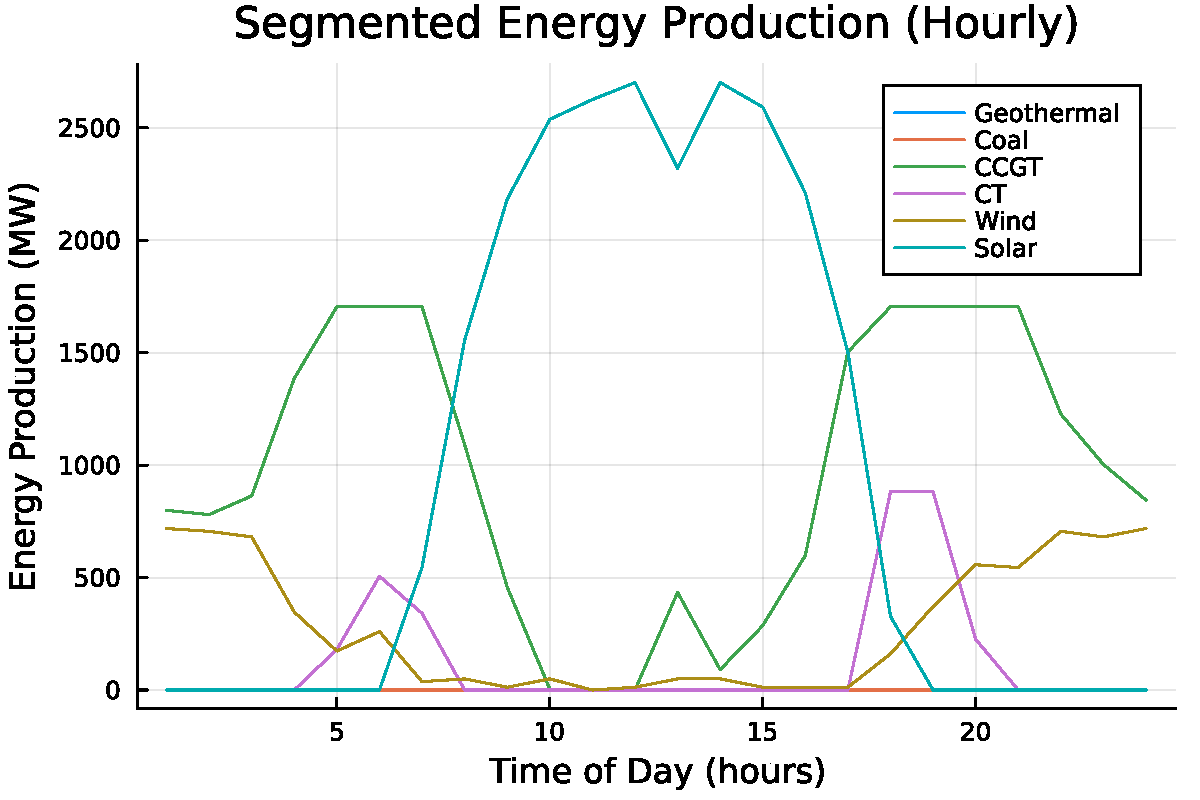
\includegraphics[width=\linewidth]{figures/solution-template_6_1.pdf}

\begin{lstlisting}
(*@\HLJLnB{julia>}@*) (*@\HLJLnf{areaplot}@*)(*@\HLJLp{((}@*)(*@\HLJLn{value}@*)(*@\HLJLoB{.}@*)(*@\HLJLp{(}@*)(*@\HLJLn{y}@*)(*@\HLJLp{)}@*)(*@\HLJLoB{.}@*)(*@\HLJLn{data}@*)(*@\HLJLp{)}@*)(*@\HLJLoB{{\textquotesingle}}@*)(*@\HLJLp{,}@*) (*@\HLJLn{title}@*) (*@\HLJLoB{=}@*) (*@\HLJLs{"{}Segmented}@*) (*@\HLJLs{Energy}@*) (*@\HLJLs{Production}@*) (*@\HLJLs{(Hourly)"{}}@*)(*@\HLJLp{,}@*) (*@\HLJLn{xlabel}@*) (*@\HLJLoB{=}@*) (*@\HLJLs{"{}Time}@*) (*@\HLJLs{of}@*) (*@\HLJLs{Day}@*) (*@\HLJLs{(hours)"{}}@*)(*@\HLJLp{,}@*)
       (*@\HLJLn{ylabel}@*) (*@\HLJLoB{=}@*) (*@\HLJLs{"{}Energy}@*) (*@\HLJLs{Production}@*) (*@\HLJLs{(MW)"{}}@*)(*@\HLJLp{,}@*) (*@\HLJLn{label}@*) (*@\HLJLoB{=}@*) (*@\HLJLnf{permutedims}@*)(*@\HLJLp{(}@*)(*@\HLJLn{Generators}@*)(*@\HLJLp{)}@*))
\end{lstlisting}
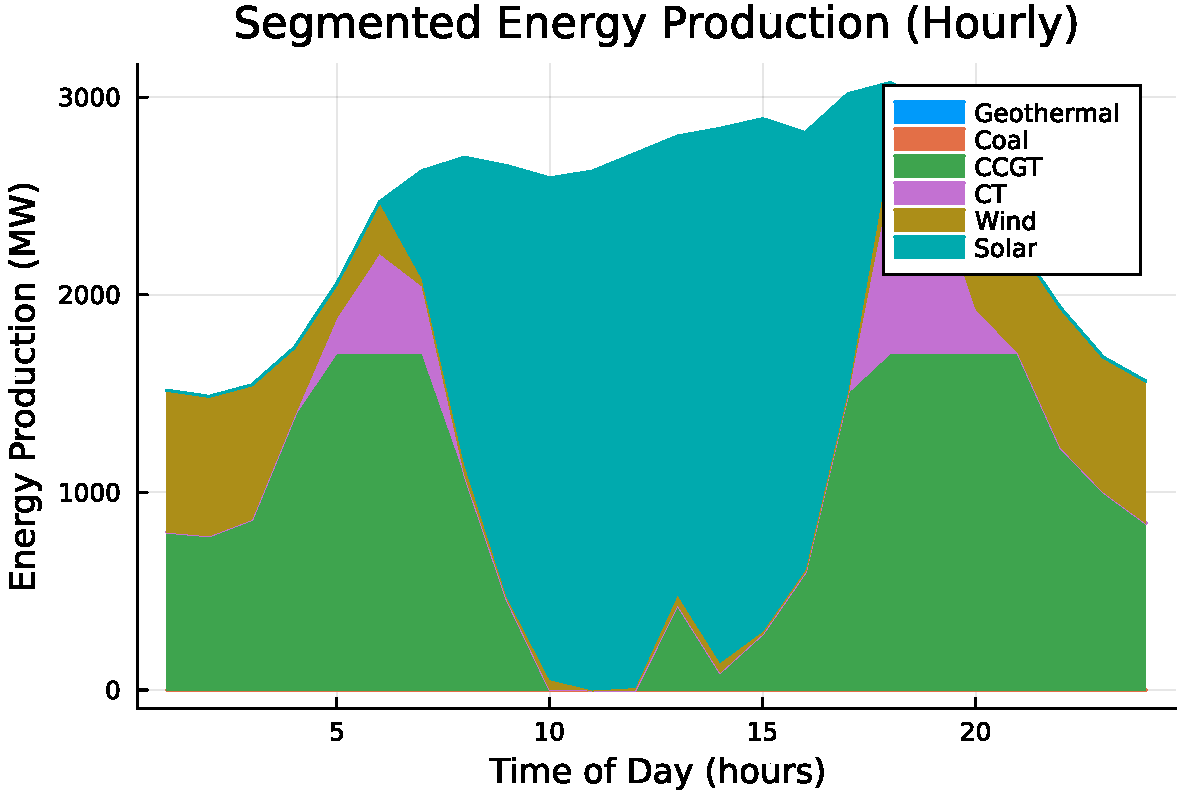
\includegraphics[width=\linewidth]{figures/solution-template_6_2.pdf}

\begin{lstlisting}
(*@\HLJLnB{julia>}@*) (*@\HLJLnf{plot!}@*)(*@\HLJLp{(}@*)(*@\HLJLn{demand}@*)(*@\HLJLp{,}@*) (*@\HLJLn{color}@*)(*@\HLJLoB{=:}@*)(*@\HLJLn{red}@*)(*@\HLJLp{,}@*) (*@\HLJLn{label}@*)(*@\HLJLoB{=}@*)(*@\HLJLs{"{}Demand"{}}@*)(*@\HLJLp{,}@*) (*@\HLJLn{linestyle}@*)(*@\HLJLoB{=:}@*)(*@\HLJLn{dash}@*))
\end{lstlisting}
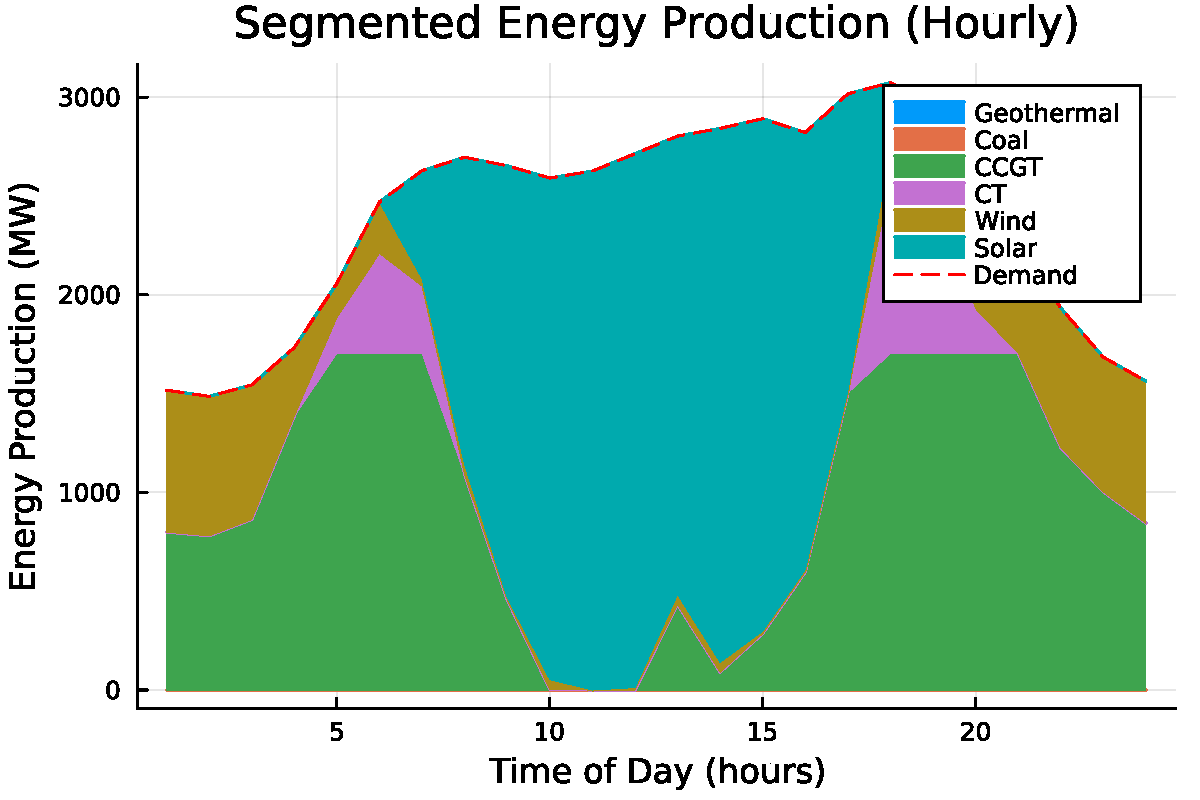
\includegraphics[width=\linewidth]{figures/solution-template_6_3.pdf}

takeaways: There exist several takeaways from this graph\_\_\_\_\_\_\_\_\_\_\_\_\_\_\_\_\_. 

\section{Problem 2}
\subsection{Problem 2.1}
This new legislation would cause us to have to add an additional constraint that limits the total amount of emissions below the legal threshold of 1.5MT of CO2. However,  the objective and decision varables will still remain the same. This new constraint can be denoted as:

\[
365 \sum_G \sum_t CO2_G \ensuremath{\leq} 1.5 \text{MT of CO2/ year}
\]
\subsection{Problem 2.2}

\begin{lstlisting}
(*@\HLJLnB{julia>}@*) (*@\HLJLn{Generators}@*) (*@\HLJLoB{=}@*) (*@\HLJLp{[}@*)(*@\HLJLs{"{}Geothermal"{}}@*)(*@\HLJLp{,}@*) (*@\HLJLs{"{}Coal"{}}@*)(*@\HLJLp{,}@*) (*@\HLJLs{"{}CCGT"{}}@*)(*@\HLJLp{,}@*) (*@\HLJLs{"{}CT"{}}@*)(*@\HLJLp{,}@*) (*@\HLJLs{"{}Wind"{}}@*)(*@\HLJLp{,}@*) (*@\HLJLs{"{}Solar"{}}@*)(*@\HLJLp{];}@*)

(*@\HLJLnB{julia>}@*) (*@\HLJLn{G}@*) (*@\HLJLoB{=}@*) (*@\HLJLni{1}@*)(*@\HLJLoB{:}@*)(*@\HLJLnf{length}@*)(*@\HLJLp{(}@*)(*@\HLJLn{Generators}@*)(*@\HLJLp{);}@*)

(*@\HLJLnB{julia>}@*) (*@\HLJLn{T}@*)(*@\HLJLoB{=}@*) (*@\HLJLn{hours}@*)(*@\HLJLp{;}@*)

(*@\HLJLnB{julia>}@*) (*@\HLJLn{Q2}@*) (*@\HLJLoB{=}@*) (*@\HLJLnf{Model}@*)(*@\HLJLp{(}@*)(*@\HLJLn{HiGHS}@*)(*@\HLJLoB{.}@*)(*@\HLJLn{Optimizer}@*)(*@\HLJLp{);}@*)

(*@\HLJLnB{julia>}@*) (*@\HLJLn{nseCost}@*) (*@\HLJLoB{=}@*) (*@\HLJLni{1000}@*)(*@\HLJLp{;}@*)

(*@\HLJLnB{julia>}@*) (*@\HLJLn{maxP}@*) (*@\HLJLoB{=}@*) (*@\HLJLnfB{1.5}@*)(*@\HLJLoB{*}@*)(*@\HLJLni{10}@*)(*@\HLJLoB{{\textasciicircum}}@*)(*@\HLJLni{6}@*)(*@\HLJLp{;}@*)

(*@\HLJLnB{julia>}@*) (*@\HLJLnd{@variable}@*)(*@\HLJLp{(}@*)(*@\HLJLn{Q2}@*)(*@\HLJLp{,}@*) (*@\HLJLn{x}@*)(*@\HLJLp{[}@*)(*@\HLJLn{G}@*)(*@\HLJLp{]}@*)(*@\HLJLoB{>=}@*)(*@\HLJLni{0}@*)(*@\HLJLp{);}@*)

(*@\HLJLnB{julia>}@*) (*@\HLJLnd{@variable}@*)(*@\HLJLp{(}@*)(*@\HLJLn{Q2}@*)(*@\HLJLp{,}@*) (*@\HLJLn{y}@*)(*@\HLJLp{[}@*)(*@\HLJLn{G}@*)(*@\HLJLp{,}@*)(*@\HLJLn{T}@*)(*@\HLJLp{]}@*) (*@\HLJLoB{>=}@*) (*@\HLJLni{0}@*)(*@\HLJLp{);}@*)

(*@\HLJLnB{julia>}@*) (*@\HLJLnd{@variable}@*)(*@\HLJLp{(}@*)(*@\HLJLn{Q2}@*)(*@\HLJLp{,}@*) (*@\HLJLn{n}@*)(*@\HLJLp{[}@*)(*@\HLJLn{T}@*)(*@\HLJLp{]}@*) (*@\HLJLoB{>=}@*)(*@\HLJLni{0}@*)(*@\HLJLp{);}@*)

(*@\HLJLnB{julia>}@*) (*@\HLJLnd{@objective}@*)(*@\HLJLp{(}@*)(*@\HLJLn{Q2}@*)(*@\HLJLp{,}@*) (*@\HLJLn{Min}@*)(*@\HLJLp{,}@*) (*@\HLJLn{investment{\_}cost}@*)(*@\HLJLoB{{\textquotesingle}*}@*) (*@\HLJLn{x}@*) (*@\HLJLoB{+}@*) (*@\HLJLni{365}@*)(*@\HLJLoB{*}@*)(*@\HLJLp{(}@*)(*@\HLJLnf{sum}@*)(*@\HLJLp{(}@*)(*@\HLJLn{op{\_}cost}@*)(*@\HLJLoB{{\textquotesingle}*}@*)(*@\HLJLn{y}@*)(*@\HLJLp{)}@*) (*@\HLJLoB{+}@*) (*@\HLJLnf{sum}@*)(*@\HLJLp{(}@*)(*@\HLJLn{n}@*)(*@\HLJLp{)}@*)(*@\HLJLoB{*}@*)(*@\HLJLn{nseCost}@*)(*@\HLJLp{))}@*)
457000 x[1] + 268000 x[2] + 85000 x[3] + 62580 x[4] + 92000 x[5] + 92000 x[6] + 8030 y[2,1] + 12775 y[3,1] + 16425 y[4,1] + 8030 y[2,2] + 12775 y[3,2] + 16425 y[4,2] + 8030 y[2,3] + 12775 y[3,3] + 16425 y[4,3] + 8030 y[2,4] + 12775 y[3,4] + 16425 y[4,4] + 8030 y[2,5] + 12775 y[3,5] + 16425 y[4,5] + 8030 y[2,6] + 12775 y[3,6] + 16425 y[4,6] + 8030 y[2,7] + 12775 y[3,7] + 16425 y[4,7] + 8030 y[2,8] + 12775 y[3,8] + 16425 y[4,8] + 8030 y[2,9] + 12775 y[3,9] + 16425 y[4,9] + 8030 y[2,10] + 12775 y[3,10] + 16425 y[4,10] + 8030 y[2,11] + 12775 y[3,11] + 16425 y[4,11] + 8030 y[2,12] + 12775 y[3,12] + 16425 y[4,12] + 8030 y[2,13] + 12775 y[3,13] + 16425 y[4,13] + 8030 y[2,14] + 12775 y[3,14] + 16425 y[4,14] + 8030 y[2,15] + 12775 y[3,15] + 16425 y[4,15] + 8030 y[2,16] + 12775 y[3,16] + 16425 y[4,16] + 8030 y[2,17] + 12775 y[3,17] + 16425 y[4,17] + 8030 y[2,18] + 12775 y[3,18] + 16425 y[4,18] + 8030 y[2,19] + 12775 y[3,19] + 16425 y[4,19] + 8030 y[2,20] + 12775 y[3,20] + 16425 y[4,20] + 8030 y[2,21] + 12775 y[3,21] + 16425 y[4,21] + 8030 y[2,22] + 12775 y[3,22] + 16425 y[4,22] + 8030 y[2,23] + 12775 y[3,23] + 16425 y[4,23] + 8030 y[2,24] + 12775 y[3,24] + 16425 y[4,24] + 365000 n[1] + 365000 n[2] + 365000 n[3] + 365000 n[4] + 365000 n[5] + 365000 n[6] + 365000 n[7] + 365000 n[8] + 365000 n[9] + 365000 n[10] + 365000 n[11] + 365000 n[12] + 365000 n[13] + 365000 n[14] + 365000 n[15] + 365000 n[16] + 365000 n[17] + 365000 n[18] + 365000 n[19] + 365000 n[20] + 365000 n[21] + 365000 n[22] + 365000 n[23] + 365000 n[24]

(*@\HLJLnB{julia>}@*) (*@\HLJLn{available}@*) (*@\HLJLoB{=}@*) (*@\HLJLnf{zeros}@*)(*@\HLJLp{(}@*)(*@\HLJLnf{length}@*)(*@\HLJLp{(}@*)(*@\HLJLn{G}@*)(*@\HLJLp{),}@*) (*@\HLJLnf{length}@*)(*@\HLJLp{(}@*)(*@\HLJLn{T}@*)(*@\HLJLp{));}@*)

(*@\HLJLnB{julia>}@*) (*@\HLJLn{available}@*)(*@\HLJLp{[}@*)(*@\HLJLni{1}@*)(*@\HLJLp{,}@*)(*@\HLJLoB{:}@*)(*@\HLJLp{]}@*) (*@\HLJLoB{.=}@*)(*@\HLJLn{thermal{\_}cf}@*)(*@\HLJLp{[}@*)(*@\HLJLni{1}@*)(*@\HLJLp{];}@*)

(*@\HLJLnB{julia>}@*) (*@\HLJLn{available}@*)(*@\HLJLp{[}@*)(*@\HLJLni{2}@*)(*@\HLJLp{,}@*)(*@\HLJLoB{:}@*)(*@\HLJLp{]}@*) (*@\HLJLoB{.=}@*)(*@\HLJLn{thermal{\_}cf}@*)(*@\HLJLp{[}@*)(*@\HLJLni{2}@*)(*@\HLJLp{];}@*)

(*@\HLJLnB{julia>}@*) (*@\HLJLn{available}@*)(*@\HLJLp{[}@*)(*@\HLJLni{3}@*)(*@\HLJLp{,}@*)(*@\HLJLoB{:}@*)(*@\HLJLp{]}@*) (*@\HLJLoB{.=}@*)(*@\HLJLn{thermal{\_}cf}@*)(*@\HLJLp{[}@*)(*@\HLJLni{3}@*)(*@\HLJLp{];}@*)

(*@\HLJLnB{julia>}@*) (*@\HLJLn{available}@*)(*@\HLJLp{[}@*)(*@\HLJLni{4}@*)(*@\HLJLp{,}@*)(*@\HLJLoB{:}@*)(*@\HLJLp{]}@*) (*@\HLJLoB{.=}@*)(*@\HLJLn{thermal{\_}cf}@*)(*@\HLJLp{[}@*)(*@\HLJLni{4}@*)(*@\HLJLp{];}@*)

(*@\HLJLnB{julia>}@*) (*@\HLJLn{available}@*)(*@\HLJLp{[}@*)(*@\HLJLni{5}@*)(*@\HLJLp{,}@*)(*@\HLJLoB{:}@*)(*@\HLJLp{]}@*) (*@\HLJLoB{.=}@*)(*@\HLJLn{wind{\_}cf}@*)(*@\HLJLp{;}@*)

(*@\HLJLnB{julia>}@*) (*@\HLJLn{available}@*)(*@\HLJLp{[}@*)(*@\HLJLni{6}@*)(*@\HLJLp{,}@*)(*@\HLJLoB{:}@*)(*@\HLJLp{]}@*) (*@\HLJLoB{.=}@*)(*@\HLJLn{solar{\_}cf}@*)(*@\HLJLp{;}@*)

(*@\HLJLnB{julia>}@*) (*@\HLJLnd{@constraint}@*)(*@\HLJLp{(}@*)(*@\HLJLn{Q2}@*)(*@\HLJLp{,}@*)(*@\HLJLn{avail}@*)(*@\HLJLp{[}@*)(*@\HLJLn{g}@*) (*@\HLJLkp{in}@*) (*@\HLJLn{G}@*)(*@\HLJLp{,}@*) (*@\HLJLn{t}@*) (*@\HLJLkp{in}@*) (*@\HLJLn{T}@*)(*@\HLJLp{],}@*)(*@\HLJLn{y}@*)(*@\HLJLp{[}@*)(*@\HLJLn{g}@*)(*@\HLJLp{,}@*)(*@\HLJLn{t}@*)(*@\HLJLp{]}@*) (*@\HLJLoB{<=}@*) (*@\HLJLn{available}@*)(*@\HLJLp{[}@*)(*@\HLJLn{g}@*)(*@\HLJLp{,}@*)(*@\HLJLn{t}@*)(*@\HLJLp{]}@*) (*@\HLJLoB{*}@*)(*@\HLJLn{x}@*)(*@\HLJLp{[}@*)(*@\HLJLn{g}@*)(*@\HLJLp{]);}@*)

(*@\HLJLnB{julia>}@*) (*@\HLJLnd{@constraint}@*)(*@\HLJLp{(}@*)(*@\HLJLn{Q2}@*)(*@\HLJLp{,}@*) (*@\HLJLn{load}@*)(*@\HLJLp{[}@*)(*@\HLJLn{t}@*) (*@\HLJLkp{in}@*) (*@\HLJLn{T}@*)(*@\HLJLp{],}@*) (*@\HLJLnf{sum}@*)(*@\HLJLp{(}@*)(*@\HLJLn{y}@*)(*@\HLJLp{[}@*)(*@\HLJLoB{:}@*)(*@\HLJLp{,}@*)(*@\HLJLn{t}@*)(*@\HLJLp{])}@*)(*@\HLJLoB{+}@*) (*@\HLJLn{n}@*)(*@\HLJLp{[}@*)(*@\HLJLn{t}@*)(*@\HLJLp{]}@*) (*@\HLJLoB{==}@*) (*@\HLJLn{demand}@*)(*@\HLJLp{[}@*)(*@\HLJLn{t}@*)(*@\HLJLp{]);}@*)

(*@\HLJLnB{julia>}@*) (*@\HLJLnd{@constraint}@*)(*@\HLJLp{(}@*)(*@\HLJLn{Q2}@*)(*@\HLJLp{,}@*) (*@\HLJLn{pollution}@*)(*@\HLJLp{[}@*)(*@\HLJLn{g}@*) (*@\HLJLkp{in}@*) (*@\HLJLn{G}@*)(*@\HLJLp{],}@*) (*@\HLJLni{365}@*)(*@\HLJLoB{*}@*)(*@\HLJLp{(}@*)(*@\HLJLnf{sum}@*)(*@\HLJLp{(}@*)(*@\HLJLn{y}@*)(*@\HLJLp{[}@*)(*@\HLJLn{g}@*)(*@\HLJLp{,}@*)(*@\HLJLoB{:}@*)(*@\HLJLp{])}@*)(*@\HLJLoB{*}@*)(*@\HLJLn{co2{\_}emissions}@*)(*@\HLJLp{[}@*)(*@\HLJLn{g}@*)(*@\HLJLp{])}@*) (*@\HLJLoB{<=}@*) (*@\HLJLn{maxP}@*)(*@\HLJLp{);}@*)

(*@\HLJLnB{julia>}@*) (*@\HLJLnf{set{\_}silent}@*)(*@\HLJLp{(}@*)(*@\HLJLn{Q2}@*))
\end{lstlisting}

\subsection{Problem 2.3}

\begin{lstlisting}
(*@\HLJLnB{julia>}@*) (*@\HLJLnf{optimize!}@*)(*@\HLJLp{(}@*)(*@\HLJLn{Q2}@*)(*@\HLJLp{)}@*)

(*@\HLJLnB{julia>}@*) (*@\HLJLn{total{\_}cost}@*) (*@\HLJLoB{=}@*) (*@\HLJLnf{objective{\_}value}@*)(*@\HLJLp{(}@*)(*@\HLJLn{Q2}@*)(*@\HLJLp{)}@*)
9.339884532803347e8

(*@\HLJLnB{julia>}@*) (*@\HLJLn{energy{\_}sources}@*) (*@\HLJLoB{=}@*) (*@\HLJLp{(}@*)(*@\HLJLn{value}@*)(*@\HLJLoB{.}@*)(*@\HLJLp{(}@*)(*@\HLJLn{x}@*)(*@\HLJLp{))}@*)
1-dimensional DenseAxisArray(*@{{\{}}@*)Float64,1,...(*@{{\}}}@*) with index sets:
    Dimension 1, 1:6
And data, a 6-element Vector(*@{{\{}}@*)Float64(*@{{\}}}@*):
    0.0
    0.0
  813.7901170184164
 1551.4733364332083
 2668.6812691819837
 3015.0665129559793

(*@\HLJLnB{julia>}@*) (*@\HLJLn{notserved}@*)(*@\HLJLoB{=}@*) (*@\HLJLnf{sum}@*)(*@\HLJLp{(}@*)(*@\HLJLn{value}@*)(*@\HLJLoB{.}@*)(*@\HLJLp{(}@*)(*@\HLJLn{n}@*)(*@\HLJLp{))}@*)
0.0

(*@\HLJLnB{julia>}@*) (*@\HLJLn{value}@*)(*@\HLJLoB{.}@*)(*@\HLJLp{(}@*)(*@\HLJLn{y}@*)(*@\HLJLp{)}@*)
2-dimensional DenseAxisArray(*@{{\{}}@*)Float64,2,...(*@{{\}}}@*) with index sets:
    Dimension 1, 1:6
    Dimension 2, 1:24
And data, a 6(*@\ensuremath{\times}@*)24 Matrix(*@{{\{}}@*)Float64(*@{{\}}}@*):
    0.0     0.0    -0.0      -0.0    (*@\ensuremath{\ldots}@*)    -0.0      -0.0      -0.0
    0.0     0.0    -0.0      -0.0         -0.0      -0.0      -0.0
    0.0     0.0    76.2253  813.79       411.852   216.225    15.1649
    0.0     0.0     0.0     171.979        0.0       0.0       0.0
 1517.0  1486.0  1467.77    747.231     1521.15   1467.77   1547.84
    0.0     0.0    -0.0      -0.0    (*@\ensuremath{\ldots}@*)    -0.0      -0.0      -0.0

(*@\HLJLnB{julia>}@*) (*@\HLJLnf{println}@*)(*@\HLJLp{(}@*)(*@\HLJLnf{round}@*)(*@\HLJLp{(}@*)(*@\HLJLn{energy{\_}sources}@*)(*@\HLJLp{[}@*)(*@\HLJLni{1}@*)(*@\HLJLp{],}@*) (*@\HLJLn{digits}@*) (*@\HLJLoB{=}@*)(*@\HLJLni{3}@*)(*@\HLJLp{),}@*) (*@\HLJLs{"{}}@*) (*@\HLJLs{MW}@*) (*@\HLJLs{via}@*) (*@\HLJLs{Geothermal}@*) (*@\HLJLs{Production."{}}@*)(*@\HLJLp{);}@*)
0.0 MW via Geothermal Production.

(*@\HLJLnB{julia>}@*) (*@\HLJLnf{println}@*)(*@\HLJLp{(}@*)(*@\HLJLnf{round}@*)(*@\HLJLp{(}@*)(*@\HLJLn{energy{\_}sources}@*)(*@\HLJLp{[}@*)(*@\HLJLni{2}@*)(*@\HLJLp{],}@*) (*@\HLJLn{digits}@*) (*@\HLJLoB{=}@*)(*@\HLJLni{3}@*)(*@\HLJLp{),}@*) (*@\HLJLs{"{}}@*) (*@\HLJLs{MW}@*) (*@\HLJLs{via}@*) (*@\HLJLs{Coal}@*) (*@\HLJLs{Production."{}}@*)(*@\HLJLp{);}@*)
0.0 MW via Coal Production.

(*@\HLJLnB{julia>}@*) (*@\HLJLnf{println}@*)(*@\HLJLp{(}@*)(*@\HLJLnf{round}@*)(*@\HLJLp{(}@*)(*@\HLJLn{energy{\_}sources}@*)(*@\HLJLp{[}@*)(*@\HLJLni{3}@*)(*@\HLJLp{],}@*) (*@\HLJLn{digits}@*) (*@\HLJLoB{=}@*)(*@\HLJLni{3}@*)(*@\HLJLp{),}@*) (*@\HLJLs{"{}}@*) (*@\HLJLs{MW}@*) (*@\HLJLs{via}@*) (*@\HLJLs{CCGT}@*) (*@\HLJLs{Production."{}}@*)(*@\HLJLp{);}@*)
813.79 MW via CCGT Production.

(*@\HLJLnB{julia>}@*) (*@\HLJLnf{println}@*)(*@\HLJLp{(}@*)(*@\HLJLnf{round}@*)(*@\HLJLp{(}@*)(*@\HLJLn{energy{\_}sources}@*)(*@\HLJLp{[}@*)(*@\HLJLni{4}@*)(*@\HLJLp{],}@*) (*@\HLJLn{digits}@*) (*@\HLJLoB{=}@*)(*@\HLJLni{3}@*)(*@\HLJLp{),}@*) (*@\HLJLs{"{}}@*) (*@\HLJLs{MW}@*) (*@\HLJLs{via}@*) (*@\HLJLs{CT}@*) (*@\HLJLs{Production."{}}@*)(*@\HLJLp{);}@*)
1551.473 MW via CT Production.

(*@\HLJLnB{julia>}@*) (*@\HLJLnf{println}@*)(*@\HLJLp{(}@*)(*@\HLJLnf{round}@*)(*@\HLJLp{(}@*)(*@\HLJLn{energy{\_}sources}@*)(*@\HLJLp{[}@*)(*@\HLJLni{5}@*)(*@\HLJLp{],}@*) (*@\HLJLn{digits}@*) (*@\HLJLoB{=}@*)(*@\HLJLni{3}@*)(*@\HLJLp{),}@*) (*@\HLJLs{"{}}@*) (*@\HLJLs{MW}@*) (*@\HLJLs{via}@*) (*@\HLJLs{Wind}@*) (*@\HLJLs{Production."{}}@*)(*@\HLJLp{);}@*)
2668.681 MW via Wind Production.

(*@\HLJLnB{julia>}@*) (*@\HLJLnf{println}@*)(*@\HLJLp{(}@*)(*@\HLJLnf{round}@*)(*@\HLJLp{(}@*)(*@\HLJLn{energy{\_}sources}@*)(*@\HLJLp{[}@*)(*@\HLJLni{6}@*)(*@\HLJLp{],}@*) (*@\HLJLn{digits}@*) (*@\HLJLoB{=}@*)(*@\HLJLni{3}@*)(*@\HLJLp{),}@*) (*@\HLJLs{"{}}@*) (*@\HLJLs{MW}@*) (*@\HLJLs{via}@*) (*@\HLJLs{Solar}@*) (*@\HLJLs{Production."{}}@*)(*@\HLJLp{);}@*)
3015.067 MW via Solar Production.

(*@\HLJLnB{julia>}@*) (*@\HLJLnf{println}@*)(*@\HLJLp{(}@*)(*@\HLJLs{"{}Total}@*) (*@\HLJLs{annual}@*) (*@\HLJLs{cost}@*) (*@\HLJLs{is}@*) (*@\HLJLse{{\textbackslash}{\$}}@*)(*@\HLJLs{"{}}@*)(*@\HLJLp{,}@*) (*@\HLJLnf{round}@*)(*@\HLJLp{(}@*)(*@\HLJLn{total{\_}cost}@*)(*@\HLJLp{,}@*) (*@\HLJLn{digits}@*) (*@\HLJLoB{=}@*) (*@\HLJLni{5}@*)(*@\HLJLp{));}@*)
Total annual cost is (*@{{\$}}@*)9.3398845328033e8

(*@\HLJLnB{julia>}@*) (*@\HLJLnf{println}@*)(*@\HLJLp{(}@*)(*@\HLJLn{notserved}@*)(*@\HLJLp{,}@*) (*@\HLJLs{"{}}@*) (*@\HLJLs{MW}@*) (*@\HLJLs{of}@*) (*@\HLJLs{energy}@*) (*@\HLJLs{goes}@*) (*@\HLJLs{non-served."{}}@*)(*@\HLJLp{);}@*)
0.0 MW of energy goes non-served.
\end{lstlisting}

Differences:

\subsection{Problem 2.4}

\begin{lstlisting}
(*@\HLJLnB{julia>}@*) (*@\HLJLnf{plot}@*)(*@\HLJLp{((}@*)(*@\HLJLn{value}@*)(*@\HLJLoB{.}@*)(*@\HLJLp{(}@*)(*@\HLJLn{y}@*)(*@\HLJLp{)}@*)(*@\HLJLoB{.}@*)(*@\HLJLn{data}@*)(*@\HLJLp{)}@*)(*@\HLJLoB{{\textquotesingle}}@*)(*@\HLJLp{,}@*) (*@\HLJLn{title}@*) (*@\HLJLoB{=}@*) (*@\HLJLs{"{}Segmented}@*) (*@\HLJLs{Energy}@*) (*@\HLJLs{Production}@*)(*@\HLJLse{{\textbackslash}n}@*) (*@\HLJLs{with}@*) (*@\HLJLs{Emissions}@*) (*@\HLJLs{Cap}@*) (*@\HLJLs{(Hourly)"{}}@*)(*@\HLJLp{,}@*) (*@\HLJLn{xlabel}@*) (*@\HLJLoB{=}@*) (*@\HLJLs{"{}Time}@*) (*@\HLJLs{of}@*) (*@\HLJLs{Day}@*) (*@\HLJLs{(hours)"{}}@*)(*@\HLJLp{,}@*)
       (*@\HLJLn{ylabel}@*) (*@\HLJLoB{=}@*) (*@\HLJLs{"{}Energy}@*) (*@\HLJLs{Production}@*) (*@\HLJLs{(MW)"{}}@*)(*@\HLJLp{,}@*) (*@\HLJLn{label}@*) (*@\HLJLoB{=}@*) (*@\HLJLnf{permutedims}@*)(*@\HLJLp{(}@*)(*@\HLJLn{Generators}@*)(*@\HLJLp{)}@*))
\end{lstlisting}
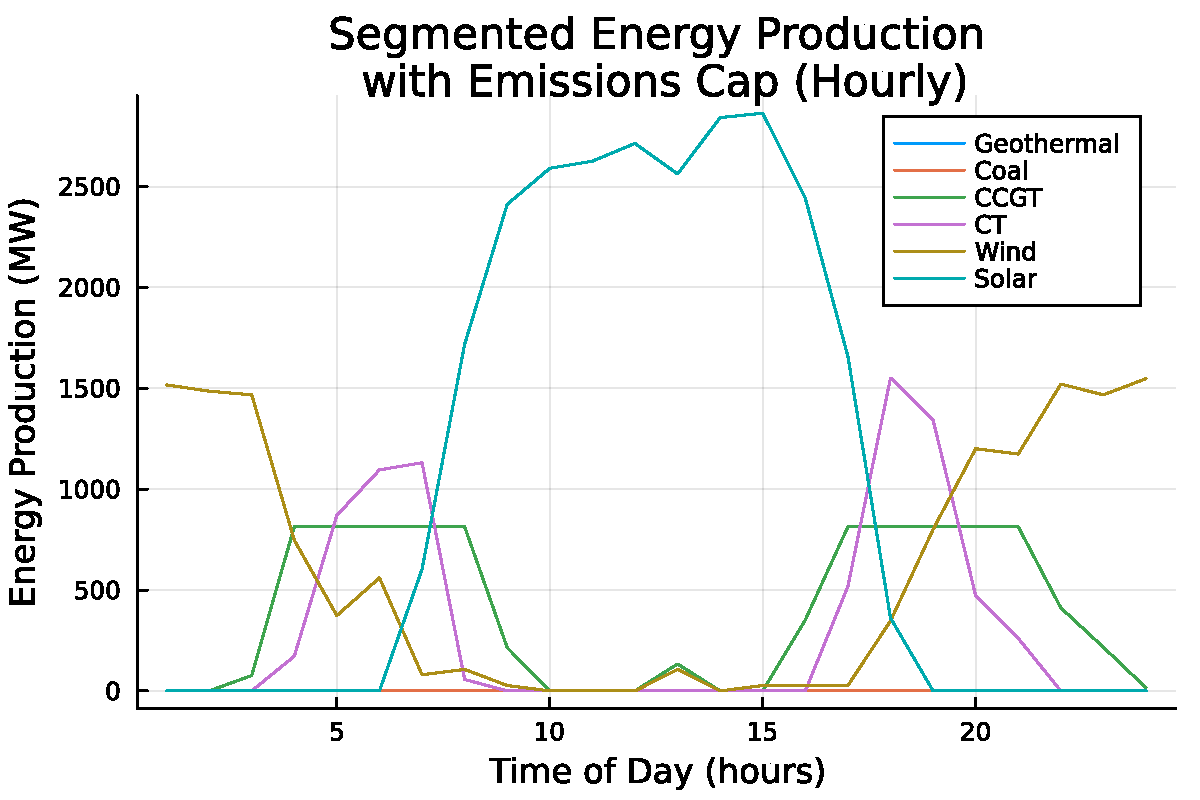
\includegraphics[width=\linewidth]{figures/solution-template_9_1.pdf}

\begin{lstlisting}
(*@\HLJLnB{julia>}@*) (*@\HLJLnf{areaplot}@*)(*@\HLJLp{((}@*)(*@\HLJLn{value}@*)(*@\HLJLoB{.}@*)(*@\HLJLp{(}@*)(*@\HLJLn{y}@*)(*@\HLJLp{)}@*)(*@\HLJLoB{.}@*)(*@\HLJLn{data}@*)(*@\HLJLp{)}@*)(*@\HLJLoB{{\textquotesingle}}@*)(*@\HLJLp{,}@*) (*@\HLJLn{title}@*) (*@\HLJLoB{=}@*) (*@\HLJLs{"{}Segmented}@*) (*@\HLJLs{Energy}@*) (*@\HLJLs{Production}@*)(*@\HLJLse{{\textbackslash}n}@*) (*@\HLJLs{with}@*) (*@\HLJLs{Emissions}@*) (*@\HLJLs{Cap}@*) (*@\HLJLs{(Hourly)"{}}@*)(*@\HLJLp{,}@*) (*@\HLJLn{xlabel}@*) (*@\HLJLoB{=}@*) (*@\HLJLs{"{}Time}@*) (*@\HLJLs{of}@*) (*@\HLJLs{Day}@*) (*@\HLJLs{(hours)"{}}@*)(*@\HLJLp{,}@*)
       (*@\HLJLn{ylabel}@*) (*@\HLJLoB{=}@*) (*@\HLJLs{"{}Energy}@*) (*@\HLJLs{Production}@*) (*@\HLJLs{(MW)"{}}@*)(*@\HLJLp{,}@*) (*@\HLJLn{label}@*) (*@\HLJLoB{=}@*) (*@\HLJLnf{permutedims}@*)(*@\HLJLp{(}@*)(*@\HLJLn{Generators}@*)(*@\HLJLp{)}@*))
\end{lstlisting}
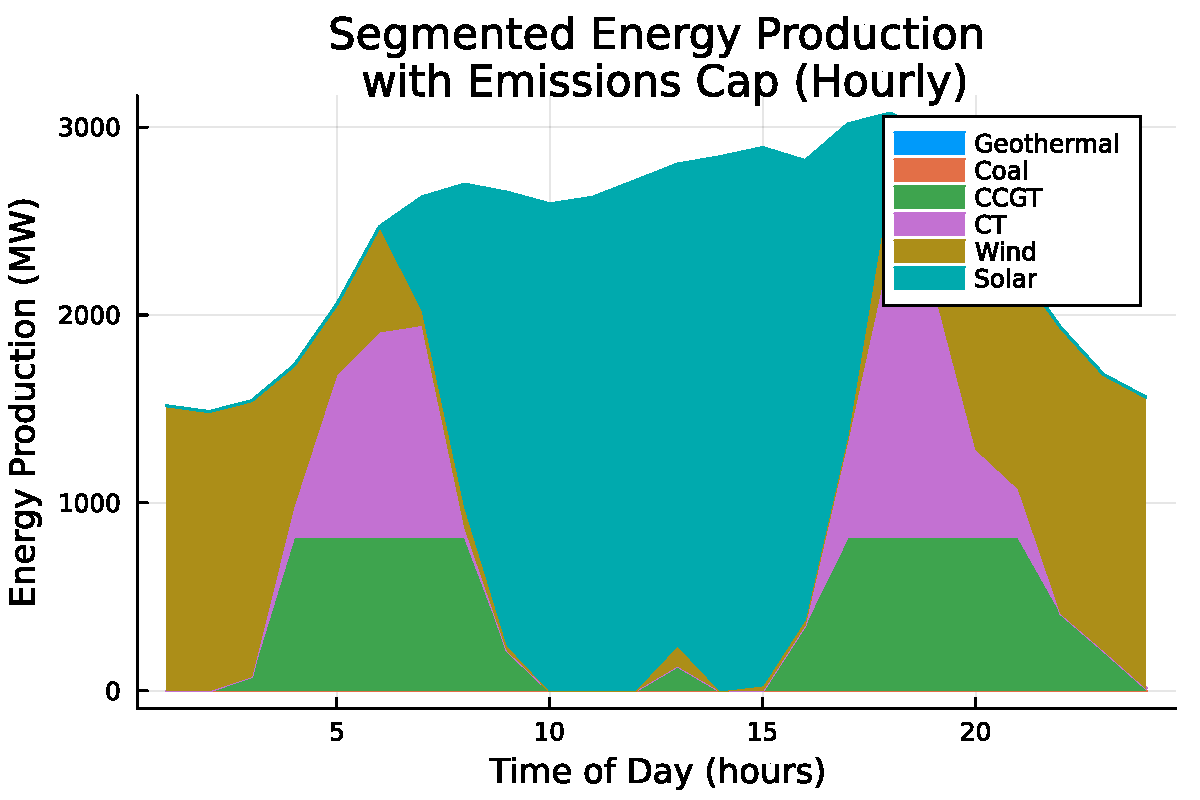
\includegraphics[width=\linewidth]{figures/solution-template_9_2.pdf}

\begin{lstlisting}
(*@\HLJLnB{julia>}@*) (*@\HLJLnf{plot!}@*)(*@\HLJLp{(}@*)(*@\HLJLn{demand}@*)(*@\HLJLp{,}@*) (*@\HLJLn{color}@*)(*@\HLJLoB{=:}@*)(*@\HLJLn{red}@*)(*@\HLJLp{,}@*) (*@\HLJLn{label}@*)(*@\HLJLoB{=}@*)(*@\HLJLs{"{}Demand"{}}@*)(*@\HLJLp{,}@*) (*@\HLJLn{linestyle}@*)(*@\HLJLoB{=:}@*)(*@\HLJLn{dash}@*))
\end{lstlisting}
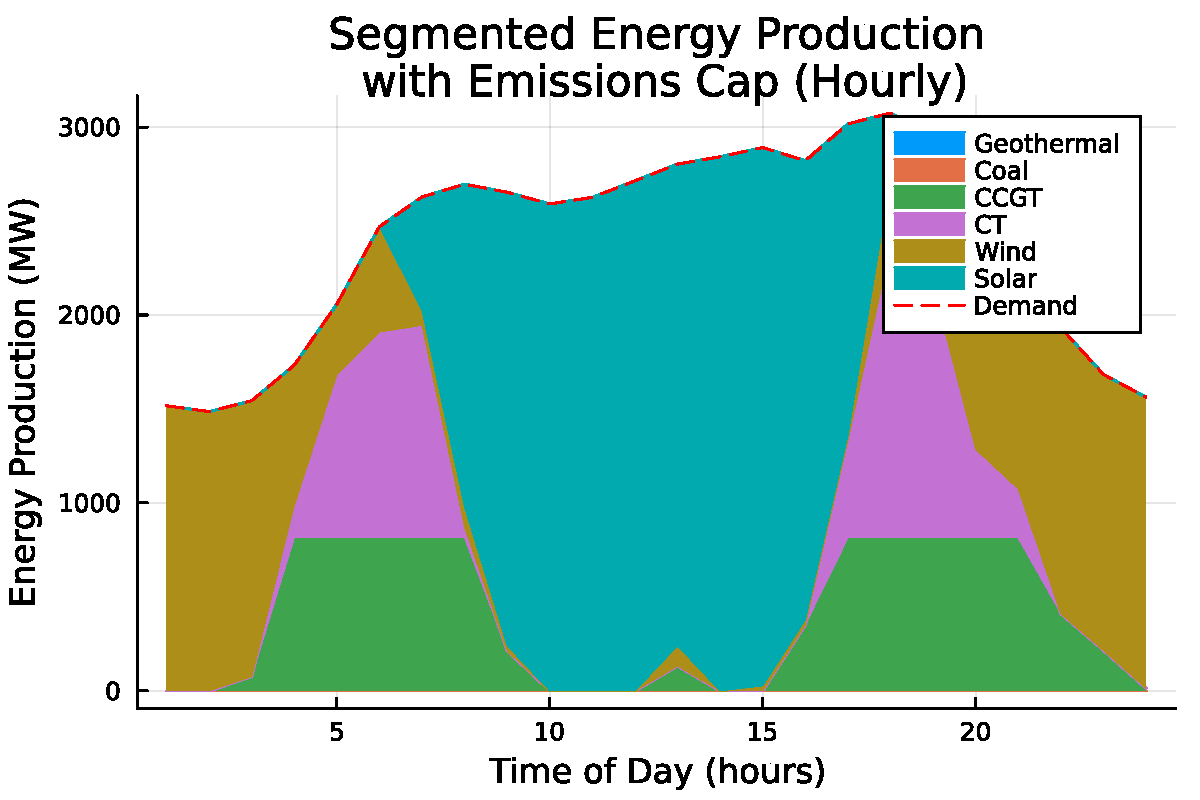
\includegraphics[width=\linewidth]{figures/solution-template_9_3.pdf}

Differences:

\subsection{Problem 2.5}

\begin{lstlisting}
(*@\HLJLnB{julia>}@*) (*@\HLJLn{Generators}@*) (*@\HLJLoB{=}@*) (*@\HLJLp{[}@*)(*@\HLJLs{"{}Geothermal"{}}@*)(*@\HLJLp{,}@*) (*@\HLJLs{"{}Coal"{}}@*)(*@\HLJLp{,}@*) (*@\HLJLs{"{}CCGT"{}}@*)(*@\HLJLp{,}@*) (*@\HLJLs{"{}CT"{}}@*)(*@\HLJLp{,}@*) (*@\HLJLs{"{}Wind"{}}@*)(*@\HLJLp{,}@*) (*@\HLJLs{"{}Solar"{}}@*)(*@\HLJLp{];}@*)

(*@\HLJLnB{julia>}@*) (*@\HLJLn{G}@*) (*@\HLJLoB{=}@*) (*@\HLJLni{1}@*)(*@\HLJLoB{:}@*)(*@\HLJLnf{length}@*)(*@\HLJLp{(}@*)(*@\HLJLn{Generators}@*)(*@\HLJLp{);}@*)

(*@\HLJLnB{julia>}@*) (*@\HLJLn{T}@*)(*@\HLJLoB{=}@*) (*@\HLJLn{hours}@*)(*@\HLJLp{;}@*)

(*@\HLJLnB{julia>}@*) (*@\HLJLn{Q2}@*) (*@\HLJLoB{=}@*) (*@\HLJLnf{Model}@*)(*@\HLJLp{(}@*)(*@\HLJLn{HiGHS}@*)(*@\HLJLoB{.}@*)(*@\HLJLn{Optimizer}@*)(*@\HLJLp{);}@*)

(*@\HLJLnB{julia>}@*) (*@\HLJLn{nseCost}@*) (*@\HLJLoB{=}@*) (*@\HLJLni{1000}@*)(*@\HLJLp{;}@*)

(*@\HLJLnB{julia>}@*) (*@\HLJLn{maxP}@*) (*@\HLJLoB{=}@*) (*@\HLJLni{1501000}@*)
1501000

(*@\HLJLnB{julia>}@*) (*@\HLJLnd{@variable}@*)(*@\HLJLp{(}@*)(*@\HLJLn{Q2}@*)(*@\HLJLp{,}@*) (*@\HLJLn{x}@*)(*@\HLJLp{[}@*)(*@\HLJLn{G}@*)(*@\HLJLp{]}@*)(*@\HLJLoB{>=}@*)(*@\HLJLni{0}@*)(*@\HLJLp{);}@*)

(*@\HLJLnB{julia>}@*) (*@\HLJLnd{@variable}@*)(*@\HLJLp{(}@*)(*@\HLJLn{Q2}@*)(*@\HLJLp{,}@*) (*@\HLJLn{y}@*)(*@\HLJLp{[}@*)(*@\HLJLn{G}@*)(*@\HLJLp{,}@*)(*@\HLJLn{T}@*)(*@\HLJLp{]}@*) (*@\HLJLoB{>=}@*) (*@\HLJLni{0}@*)(*@\HLJLp{);}@*)

(*@\HLJLnB{julia>}@*) (*@\HLJLnd{@variable}@*)(*@\HLJLp{(}@*)(*@\HLJLn{Q2}@*)(*@\HLJLp{,}@*) (*@\HLJLn{n}@*)(*@\HLJLp{[}@*)(*@\HLJLn{T}@*)(*@\HLJLp{]}@*) (*@\HLJLoB{>=}@*)(*@\HLJLni{0}@*)(*@\HLJLp{);}@*)

(*@\HLJLnB{julia>}@*) (*@\HLJLnd{@objective}@*)(*@\HLJLp{(}@*)(*@\HLJLn{Q2}@*)(*@\HLJLp{,}@*) (*@\HLJLn{Min}@*)(*@\HLJLp{,}@*) (*@\HLJLn{investment{\_}cost}@*)(*@\HLJLoB{{\textquotesingle}*}@*) (*@\HLJLn{x}@*) (*@\HLJLoB{+}@*) (*@\HLJLni{365}@*)(*@\HLJLoB{*}@*)(*@\HLJLp{(}@*)(*@\HLJLnf{sum}@*)(*@\HLJLp{(}@*)(*@\HLJLn{op{\_}cost}@*)(*@\HLJLoB{{\textquotesingle}*}@*)(*@\HLJLn{y}@*)(*@\HLJLp{)}@*) (*@\HLJLoB{+}@*) (*@\HLJLnf{sum}@*)(*@\HLJLp{(}@*)(*@\HLJLn{n}@*)(*@\HLJLp{)}@*)(*@\HLJLoB{*}@*)(*@\HLJLn{nseCost}@*)(*@\HLJLp{))}@*)
457000 x[1] + 268000 x[2] + 85000 x[3] + 62580 x[4] + 92000 x[5] + 92000 x[6] + 8030 y[2,1] + 12775 y[3,1] + 16425 y[4,1] + 8030 y[2,2] + 12775 y[3,2] + 16425 y[4,2] + 8030 y[2,3] + 12775 y[3,3] + 16425 y[4,3] + 8030 y[2,4] + 12775 y[3,4] + 16425 y[4,4] + 8030 y[2,5] + 12775 y[3,5] + 16425 y[4,5] + 8030 y[2,6] + 12775 y[3,6] + 16425 y[4,6] + 8030 y[2,7] + 12775 y[3,7] + 16425 y[4,7] + 8030 y[2,8] + 12775 y[3,8] + 16425 y[4,8] + 8030 y[2,9] + 12775 y[3,9] + 16425 y[4,9] + 8030 y[2,10] + 12775 y[3,10] + 16425 y[4,10] + 8030 y[2,11] + 12775 y[3,11] + 16425 y[4,11] + 8030 y[2,12] + 12775 y[3,12] + 16425 y[4,12] + 8030 y[2,13] + 12775 y[3,13] + 16425 y[4,13] + 8030 y[2,14] + 12775 y[3,14] + 16425 y[4,14] + 8030 y[2,15] + 12775 y[3,15] + 16425 y[4,15] + 8030 y[2,16] + 12775 y[3,16] + 16425 y[4,16] + 8030 y[2,17] + 12775 y[3,17] + 16425 y[4,17] + 8030 y[2,18] + 12775 y[3,18] + 16425 y[4,18] + 8030 y[2,19] + 12775 y[3,19] + 16425 y[4,19] + 8030 y[2,20] + 12775 y[3,20] + 16425 y[4,20] + 8030 y[2,21] + 12775 y[3,21] + 16425 y[4,21] + 8030 y[2,22] + 12775 y[3,22] + 16425 y[4,22] + 8030 y[2,23] + 12775 y[3,23] + 16425 y[4,23] + 8030 y[2,24] + 12775 y[3,24] + 16425 y[4,24] + 365000 n[1] + 365000 n[2] + 365000 n[3] + 365000 n[4] + 365000 n[5] + 365000 n[6] + 365000 n[7] + 365000 n[8] + 365000 n[9] + 365000 n[10] + 365000 n[11] + 365000 n[12] + 365000 n[13] + 365000 n[14] + 365000 n[15] + 365000 n[16] + 365000 n[17] + 365000 n[18] + 365000 n[19] + 365000 n[20] + 365000 n[21] + 365000 n[22] + 365000 n[23] + 365000 n[24]

(*@\HLJLnB{julia>}@*) (*@\HLJLn{available}@*) (*@\HLJLoB{=}@*) (*@\HLJLnf{zeros}@*)(*@\HLJLp{(}@*)(*@\HLJLnf{length}@*)(*@\HLJLp{(}@*)(*@\HLJLn{G}@*)(*@\HLJLp{),}@*) (*@\HLJLnf{length}@*)(*@\HLJLp{(}@*)(*@\HLJLn{T}@*)(*@\HLJLp{));}@*)

(*@\HLJLnB{julia>}@*) (*@\HLJLn{available}@*)(*@\HLJLp{[}@*)(*@\HLJLni{1}@*)(*@\HLJLp{,}@*)(*@\HLJLoB{:}@*)(*@\HLJLp{]}@*) (*@\HLJLoB{.=}@*)(*@\HLJLn{thermal{\_}cf}@*)(*@\HLJLp{[}@*)(*@\HLJLni{1}@*)(*@\HLJLp{];}@*)

(*@\HLJLnB{julia>}@*) (*@\HLJLn{available}@*)(*@\HLJLp{[}@*)(*@\HLJLni{2}@*)(*@\HLJLp{,}@*)(*@\HLJLoB{:}@*)(*@\HLJLp{]}@*) (*@\HLJLoB{.=}@*)(*@\HLJLn{thermal{\_}cf}@*)(*@\HLJLp{[}@*)(*@\HLJLni{2}@*)(*@\HLJLp{];}@*)

(*@\HLJLnB{julia>}@*) (*@\HLJLn{available}@*)(*@\HLJLp{[}@*)(*@\HLJLni{3}@*)(*@\HLJLp{,}@*)(*@\HLJLoB{:}@*)(*@\HLJLp{]}@*) (*@\HLJLoB{.=}@*)(*@\HLJLn{thermal{\_}cf}@*)(*@\HLJLp{[}@*)(*@\HLJLni{3}@*)(*@\HLJLp{];}@*)

(*@\HLJLnB{julia>}@*) (*@\HLJLn{available}@*)(*@\HLJLp{[}@*)(*@\HLJLni{4}@*)(*@\HLJLp{,}@*)(*@\HLJLoB{:}@*)(*@\HLJLp{]}@*) (*@\HLJLoB{.=}@*)(*@\HLJLn{thermal{\_}cf}@*)(*@\HLJLp{[}@*)(*@\HLJLni{4}@*)(*@\HLJLp{];}@*)

(*@\HLJLnB{julia>}@*) (*@\HLJLn{available}@*)(*@\HLJLp{[}@*)(*@\HLJLni{5}@*)(*@\HLJLp{,}@*)(*@\HLJLoB{:}@*)(*@\HLJLp{]}@*) (*@\HLJLoB{.=}@*)(*@\HLJLn{wind{\_}cf}@*)(*@\HLJLp{;}@*)

(*@\HLJLnB{julia>}@*) (*@\HLJLn{available}@*)(*@\HLJLp{[}@*)(*@\HLJLni{6}@*)(*@\HLJLp{,}@*)(*@\HLJLoB{:}@*)(*@\HLJLp{]}@*) (*@\HLJLoB{.=}@*)(*@\HLJLn{solar{\_}cf}@*)(*@\HLJLp{;}@*)

(*@\HLJLnB{julia>}@*) (*@\HLJLnd{@constraint}@*)(*@\HLJLp{(}@*)(*@\HLJLn{Q2}@*)(*@\HLJLp{,}@*)(*@\HLJLn{avail}@*)(*@\HLJLp{[}@*)(*@\HLJLn{g}@*) (*@\HLJLkp{in}@*) (*@\HLJLn{G}@*)(*@\HLJLp{,}@*) (*@\HLJLn{t}@*) (*@\HLJLkp{in}@*) (*@\HLJLn{T}@*)(*@\HLJLp{],}@*)(*@\HLJLn{y}@*)(*@\HLJLp{[}@*)(*@\HLJLn{g}@*)(*@\HLJLp{,}@*)(*@\HLJLn{t}@*)(*@\HLJLp{]}@*) (*@\HLJLoB{<=}@*) (*@\HLJLn{available}@*)(*@\HLJLp{[}@*)(*@\HLJLn{g}@*)(*@\HLJLp{,}@*)(*@\HLJLn{t}@*)(*@\HLJLp{]}@*) (*@\HLJLoB{*}@*)(*@\HLJLn{x}@*)(*@\HLJLp{[}@*)(*@\HLJLn{g}@*)(*@\HLJLp{]);}@*)

(*@\HLJLnB{julia>}@*) (*@\HLJLnd{@constraint}@*)(*@\HLJLp{(}@*)(*@\HLJLn{Q2}@*)(*@\HLJLp{,}@*) (*@\HLJLn{load}@*)(*@\HLJLp{[}@*)(*@\HLJLn{t}@*) (*@\HLJLkp{in}@*) (*@\HLJLn{T}@*)(*@\HLJLp{],}@*) (*@\HLJLnf{sum}@*)(*@\HLJLp{(}@*)(*@\HLJLn{y}@*)(*@\HLJLp{[}@*)(*@\HLJLoB{:}@*)(*@\HLJLp{,}@*)(*@\HLJLn{t}@*)(*@\HLJLp{])}@*)(*@\HLJLoB{+}@*) (*@\HLJLn{n}@*)(*@\HLJLp{[}@*)(*@\HLJLn{t}@*)(*@\HLJLp{]}@*) (*@\HLJLoB{==}@*) (*@\HLJLn{demand}@*)(*@\HLJLp{[}@*)(*@\HLJLn{t}@*)(*@\HLJLp{]);}@*)

(*@\HLJLnB{julia>}@*) (*@\HLJLnd{@constraint}@*)(*@\HLJLp{(}@*)(*@\HLJLn{Q2}@*)(*@\HLJLp{,}@*) (*@\HLJLn{pollution}@*)(*@\HLJLp{[}@*)(*@\HLJLn{g}@*) (*@\HLJLkp{in}@*) (*@\HLJLn{G}@*)(*@\HLJLp{],}@*) (*@\HLJLni{365}@*)(*@\HLJLoB{*}@*)(*@\HLJLp{(}@*)(*@\HLJLnf{sum}@*)(*@\HLJLp{(}@*)(*@\HLJLn{y}@*)(*@\HLJLp{[}@*)(*@\HLJLn{g}@*)(*@\HLJLp{,}@*)(*@\HLJLoB{:}@*)(*@\HLJLp{])}@*)(*@\HLJLoB{*}@*)(*@\HLJLn{co2{\_}emissions}@*)(*@\HLJLp{[}@*)(*@\HLJLn{g}@*)(*@\HLJLp{])}@*) (*@\HLJLoB{<=}@*) (*@\HLJLn{maxP}@*)(*@\HLJLp{);}@*)

(*@\HLJLnB{julia>}@*) (*@\HLJLnf{set{\_}silent}@*)(*@\HLJLp{(}@*)(*@\HLJLn{Q2}@*)(*@\HLJLp{)}@*)

(*@\HLJLnB{julia>}@*) (*@\HLJLnf{optimize!}@*)(*@\HLJLp{(}@*)(*@\HLJLn{Q2}@*)(*@\HLJLp{)}@*)

(*@\HLJLnB{julia>}@*) (*@\HLJLn{total{\_}cost1}@*) (*@\HLJLoB{=}@*) (*@\HLJLnf{objective{\_}value}@*)(*@\HLJLp{(}@*)(*@\HLJLn{Q2}@*)(*@\HLJLp{)}@*)
9.339333048215723e8

(*@\HLJLnB{julia>}@*) (*@\HLJLn{energy{\_}sources}@*) (*@\HLJLoB{=}@*) (*@\HLJLp{(}@*)(*@\HLJLn{value}@*)(*@\HLJLoB{.}@*)(*@\HLJLp{(}@*)(*@\HLJLn{x}@*)(*@\HLJLp{))}@*)
1-dimensional DenseAxisArray(*@{{\{}}@*)Float64,1,...(*@{{\}}}@*) with index sets:
    Dimension 1, 1:6
And data, a 6-element Vector(*@{{\{}}@*)Float64(*@{{\}}}@*):
    0.0
    0.0
  813.824069940046
 1551.7793552294854
 2666.040442264474
 3015.0943111340584

(*@\HLJLnB{julia>}@*) (*@\HLJLn{value}@*)(*@\HLJLoB{.}@*)(*@\HLJLp{(}@*)(*@\HLJLn{y}@*)(*@\HLJLp{)}@*)
2-dimensional DenseAxisArray(*@{{\{}}@*)Float64,2,...(*@{{\}}}@*) with index sets:
    Dimension 1, 1:6
    Dimension 2, 1:24
And data, a 6(*@\ensuremath{\times}@*)24 Matrix(*@{{\{}}@*)Float64(*@{{\}}}@*):
    0.0     0.0    -0.0      -0.0    (*@\ensuremath{\ldots}@*)    -0.0      -0.0      -0.0
    0.0     0.0    -0.0      -0.0         -0.0      -0.0      -0.0
    0.0     0.0    77.6778  813.824      413.357   217.678    16.6965
    0.0     0.0     0.0     172.685        0.0       0.0       0.0
 1517.0  1486.0  1466.32    746.491     1519.64   1466.32   1546.3
    0.0     0.0    -0.0      -0.0    (*@\ensuremath{\ldots}@*)    -0.0      -0.0      -0.0

(*@\HLJLnB{julia>}@*) (*@\HLJLn{new{\_}cost}@*) (*@\HLJLoB{=}@*) (*@\HLJLn{total{\_}cost}@*)(*@\HLJLoB{-}@*)(*@\HLJLn{total{\_}cost1}@*)
55148.4587624073

(*@\HLJLnB{julia>}@*) (*@\HLJLnf{println}@*)(*@\HLJLp{(}@*)(*@\HLJLs{"{}Value}@*) (*@\HLJLs{of}@*) (*@\HLJLs{additional}@*) (*@\HLJLs{utility}@*) (*@\HLJLs{is}@*) (*@\HLJLse{{\textbackslash}{\$}}@*)(*@\HLJLs{"{}}@*)(*@\HLJLp{,}@*) (*@\HLJLnf{round}@*)(*@\HLJLp{(}@*)(*@\HLJLn{new{\_}cost}@*)(*@\HLJLp{,}@*) (*@\HLJLn{digits}@*) (*@\HLJLoB{=}@*) (*@\HLJLni{2}@*)(*@\HLJLp{));}@*)
Value of additional utility is (*@{{\$}}@*)55148.46
\end{lstlisting}

\section{References}
I got help from Ian Shen-Costello Lectures 11 \& 13.



\end{document}